\chapter{Method}
\label{chap:method}

% This is the introduction to the thesis.\footnote{And this is a
% footnote.}  The conclusion is in Chapter on page
\section{Out-of-Vocabulary Model}
    \subsection{Sequence Feature Extraction}
        OOV problem is handled from quasi-generative perspective as
        aforementioned in chapter \nameref{chap:intro} by using neural
        language model under assumption that there is a form that
        could generate embedding for the original embedding. Hence
        that, the original vocabulary and its embedding is used for
        training the model to generate the embedding. In chapter
        \nameref{chap:intro}, reasons why \textsc{Mimick} could
        perform worse is because the OOV embedding is generated from
        the last hidden states of the bi-LSTM and the hidden states is
        controlled by cell gates $C_t$ making the information that is
        carried on is the most recent information. If at certain time
        step $t$ the cell gates decided to forget past information,
        then the early information might not be coded into the hidden
        state. On top of that, there are evidences that recurrent
        architecture could perform worse than CNN for sequence
        modelling \citep{empirical2018shaujie}. 
        
        If explained formally, when $C_t = 0$ from equation
        \ref{eq:lstm:C_t}, hidden state from equation
        \ref{eq:lstm:h_t} will also be $0$, resetting to its starting
        state, rendering hidden states prior to time $t$ gone. This
        problem can be solved by using bi-LSTM, since bi-LSTM processes
        sequence in forward and reverse order making both early and
        later sequences held by the last hidden state for each reverse
        LSTM and forward LSTM respectively. Another problem might
        arise when we need to divide sequence into more than three
        subsequence as shown on figure \ref{fig:subsequence}. Hence
        another approach is needed since intermediate subsequence
        might get deleted or carried along with the later sequences
        even with bi-LSTM. Another method that might be able to solve
        this problem for \textsc{Mimick} is by increasing hidden size
        and hope that it will be able to compensate the sequence that
        is dropped by the cell gate in the other hidden cell.
        \begin{figure}
            \begin{align*}
                &un \vert recogniz \vert able \\
                &inter \vert national \vert ities \\
                &oto \vert rhino \vert laryngolog \vert ical \\
                &hepatico \vert chol \vert angio \vert gastro \vert stomy
            \end{align*}
            \caption{Word examples with three or more subsequences}
            \label{fig:subsequence}
        \end{figure}

        \begin{figure}
            \begin{align*}
                unrecognizable : &unre \vert nrec \vert reco \vert ecog \vert cogn \vert ogni \vert gniz \vert niza \vert izab \vert zabl \vert able\\
                internationalities : &inte \vert nter \vert tern \vert erna \vert rnat \vert nati \vert atio \vert tion \vert iona \vert onal \vert \\
                &nali \vert alit \vert liti \vert itie \vert ties\\
                otorhinolaryngological : &otor \vert torh \vert orhi \vert rhin \vert hino \vert inol \vert nola \vert olar \vert lary \vert \\
                &aryn \vert ryng \vert yngo \vert ngol \vert golo \vert olog \vert logi \vert ogic \vert gica \vert ical\\
                hepaticocholangiogastrostomy : &hepa \vert epat \vert pati \vert atic \vert tico \vert icoc \vert coch \vert ocho \vert chol \vert hola \vert olan \vert\\
                &lang \vert angi \vert ngio \vert giog \vert ioga \vert ogas \vert gast \vert astr \vert stro \vert\\
                &tros \vert rost \vert osto \vert stom \vert tomy
            \end{align*}
            \caption{4-grams examples}
            \label{fig:4grams}
        \end{figure}

        For all subsequence to be processed, we need a method that
        accounts for the whole sequence yet still able to divides the
        whole sequence into subsequences. Consequently, n-grams is
        chosen because this method splits word into sequence of
        characters depends on the chosen window size as shown on
        figure \ref{fig:4grams}. Before processing the n-grams, the
        word first split into sequence of characters and then each
        character is transformed into embedding and processed with CNN
        inspired from CNN word n-grams \citep{convolutional2014kim}.
        Those sequences of character embeddings then fed into learning
        algorithm. This idea is similar to how human tries to
        recognize an unseen word by reading subword that is
        understandable beforehand when no explanation or context were
        given. In other words, given sets of vocabulary $\mathcal{V}$
        with size $\vert\mathcal{V}\vert$ and pretrained embeddings
        $\mathcal{W}^{\vert\mathcal{V}\vert \times d}$ for each word
        $w_{i} \in \mathcal{V}$ that is represented as a vector $e_i$
        with $d$ dimension, the model is trained to map function
        $f:\mathcal{V} \rightarrow \mathbb{R}^d$ that minimizes the
        loss function,
        \begin{equation}
            \label{eq:lossfn}
            \mathcal{L} = \Vert f(w_i) - e_i \Vert^{2}_2
        \end{equation}
        This approach is similar to \textsc{Mimick}
        \cite{mimicking2017Pinter} approach. The text input is
        represented as a sequence of character $[c_1, c_2, \dots,
        c_m]$ for $c_i \in \mathcal{C}$. Those sequence then
        transformed as sequence of vectors $g_i$ with $b$ dimension by
        using character embeddings $\mathcal{G}^{\vert \mathcal{C}
        \vert \times b}$. For simplicity, sequence of $[g_1, g_2,
        \dots, g_m]$ will be called $\{g\}^m$. $\{g\}^m$ becomes
        2-dimensional matrix that has size of $m \times b$. In
        summary, given word $w$ will be transformed using embedding
        generation function $h$ into $\{g\}^m$ as shown on equation
        \ref{eq:word2charemb}.

        \begin{equation}
            \label{eq:word2charemb}
            h: w \rightarrow \{g\}_1^m
        \end{equation}

        To process $\{g\}^m$ like an n-grams, CNN is used inspired
        by CNN n-grams implementation by \cite{convolutional2014kim}.
        CNN n-grams is basically a method to do convolution on matrix
        by using a kernel $k_i^{b \times n} \in K$ for $n$ is the
        window size of the grams and $b$ is the dimension size of the
        character embedding. This operation is represented with $*$
        symbol as stated in equation \ref{eq:conv_d:2}. This operation
        produced another vector $\hat{l}$ that represents the value of
        each grams, then non-linearity is applied to this vector by
        using ReLU activation,
        \begin{equation}
            \label{eq:relu}
            ReLU(x) = max(0,x)
        \end{equation}

        Several kernel is used to learn several features for producing
        embeddings. Each of these kernel will be responsible to find
        grams that are affecting the results, thus the vector
        $\hat{l_i}$ that are results of convolution $\{g\}^m * k_i$
        will be maxpooled to produce one number. In details, from
        given sequence of character embedding $\{g\}^m$, only gram
        that produces the highest value when convoluted by using
        kernel $k_i$ will be processed. Since, there are $\vert K
        \vert$ number of filter, $\vert K \vert$ number of grams will
        be considered to be important to the results. Furthermore, by
        using several window sizes for n-grams (bigram, trigram, etc.)
        by changing the size of the kernel more features will be able
        to be learned. For instance bigram will has a kernel with size
        $b \times 2$, trigram will has a kernel with size $b \times
        3$, and so on and so forth, making the different sizes of
        n-grams can be trained together only then concatenated later.

    \subsection{Embedding Generation}
        After the features are able to be extracted, those features
        then concatenated and fed into fully connected layer with
        output size matching the pretrained embedding $\mathcal{W}$
        dimension $d$ with non-linear activation function $hardtanh$
        matching the maximum and minimum bound of the pretrained
        embedding $\mathcal{W}$ resulting a new embedding vector
        $\tilde{e}$. The fully connected layer consist of one hidden
        layer and one output layer with batch normalization before
        each layer to further sped up the training convergence
        according to \cite{batchnorm:DBLP:journals/corr/IoffeS15}.
        This normalization layer basically maintain that the
        distribution of each minibatch remains similar so that
        covariance shift is minimized in the training process
        \citep{batchnorm:DBLP:journals/corr/IoffeS15}. This process
        was done by applying transformation on each minibatch to a
        certain mean and variance
        \citep{batchnorm:DBLP:journals/corr/IoffeS15}. This mean and
        variance are learnable parameters. Let minibatch $\mathcal{B}
        = {x_1, x_2, \dots, x_m}$, following operation was applied,
        \begin{align}
            \label{eq:bn:mu}
            \mu_{\mathcal{B}} &= \frac{1}{m} \sum_{i=1}^m x_i\\
            \label{eq:bn:var}
            \sigma^2_{\mathcal{B}} &= \frac{1}{m} \sum_{i=1}^m (x_i - \mu_{\mathcal{B}}^2\\
            \label{eq:bn:norm}            
            \tilde{x}_i &= \frac{x_i - \mu_{\mathcal{B}}}{\sqrt{\sigma^2_{\mathcal{B}} + \epsilon}}\\
            \label{eq:bn:transform}            
            BN(x_i) &= \gamma\tilde{x_i} + \beta
        \end{align}
        Equation \ref{eq:bn:mu} and equation \ref{eq:bn:var} tries to
        find the mean and variance to normalize the minibatch by
        equation \ref{eq:bn:norm}. After all of the data in the
        minibatch $\mathcal{B}$ was normalized, the data then scaled
        by parameter $\gamma$ and shifted by parameter $\beta$ as
        shown in equation \ref{eq:bn:transform}. By making the
        parameters $\gamma$ and $\beta$ learnable, the model will
        adjust this process in the training process.

        After all the process above was done, the generated embedding
        vector $\tilde{e}$ was produced.
        % then passed into a highway network to
        % decide whether some information should be carried or should be
        % forgotten to obtain a new sets of embedding. Given the output
        % of max-over-time pooling $m$, The highway network is
        % calculated by the following equation, 
        % \begin{align}
        %     \label{eq:highway}
        %     t &= ReLU(f(\mathbf{W}m + b))\\
        %     \mathbf{Z} &= t \odot g(\mathbf{W_{\mathbf{H}}}m + b_{\mathbf{H}}) + (1-t) \odot m
        % \end{align}
        The complete process from input word, feature extraction,
        until predicting embedding is shown on figure \ref{fig:model}.
        \begin{figure}
            \centering
            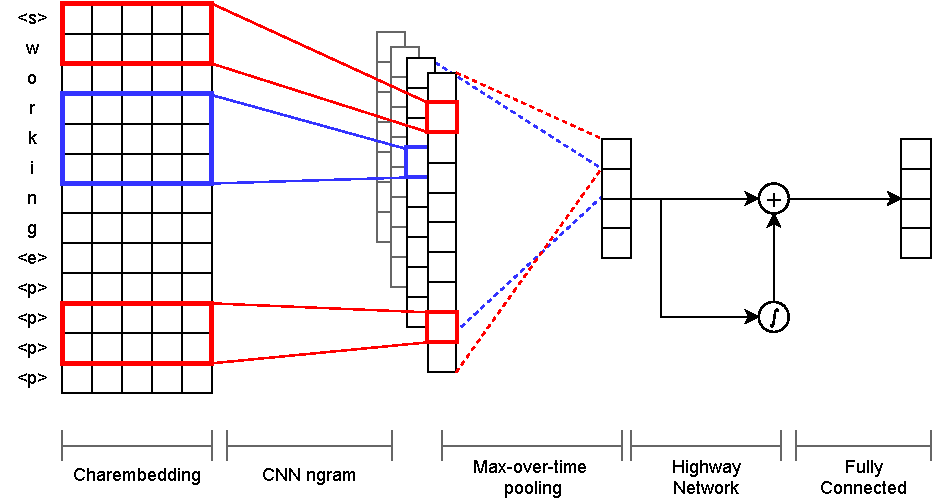
\includegraphics[width=.8\linewidth]{images/model2.pdf}
            \caption{OOV Inferencing Model}
            \label{fig:model}
        \end{figure}
        On figure \ref{fig:model}, starting and ending token is added
        at the beginning and the end of the word respectively.
        Furthermore, padding token is added if the input word is
        shorter than the longest input size in the minibatch. The
        padding token is a zero vector $\vec{0}$ and $\vec{0} * k =
        \vec{0}$ for any $k$. This is to ensure that part of input
        that got padded does not goes through maxpool layer since only
        grams that has highest value can goes through the next layer
        and minimum value of ReLU is 0 thus the result of maxpooling
        it will be 0. The reason for this is so that various length
        of words are able to be processed by the model.

    \subsection{Error and Backpropagation}
        The predicted embedding $\tilde{e}$ from the model then
        compared with the original embedding $e$ to adjust all of the
        parameters for the neural network using mean squared error
        function,
        \begin{equation}
            \label{eq:errorf}
            Error = \frac{1}{2} \Vert e - \tilde{e} \Vert ^{2}_2
        \end{equation}
        By minimizing $Error$ it is similar by minimizing
        $\mathcal{L}$ shown in equation \ref{eq:lossfn}. The error
        then backpropagated to fine-tune the neural network
        parameters, character embedding $\mathcal{G}$, the kernel $k
        \in K$, and the batch normalization parameters $\gamma and
        \beta$.
        
\section{Measuring Performance on Downstream Tasks}
    In natural language modeling (NLP), there are several tasks that
    make use of word embedding. Hence that, the generated embeddings
    from the model can be evaluated by using those downstream tasks.
    The results then compared with the state-of-the-art OOV handling
    model \textsc{Mimick} \citep{mimicking2017Pinter}.
    
    \subsection{Part-of-Speech Tagging}
        Part-of-speech tagging or POS-tagging is a task of classifying
        usage of words in sentence or corpus based on the grammatical
        usage of the word \{CITE\}, for example: verb, noun, adverb,
        etc. Given sentence $S = \{w \in \mathcal{V} \vert ((w_1,
        t_1), (w_2, t_2)\\, \dots, (w_n, t_n)\}$ with its POS-tag
        $t_i$, each word $w_i$ that exist in the vocabulary $w_i \in
        \mathcal{V}$ and $w_i \in S$ is transformed into embedding
        $e_i$. For the OOV, every sequence of the characters building
        a word transformed into sequence of character embedding
        $\{g\}_{i}^m$ using model represented in equation
        \ref{eq:word2charemb} then the embedding $\tilde{e}_i$ is
        predicted using the OOV handling model, else the original
        embedding is used if the word exist inside the vocabulary
        $\mathcal{V}$. This was done by masking the output of the OOV
        handling model and the original embedding in the following
        way,
        \begin{align}
            \label{eq:embeddingmask}
            embedding &= mask \odot e_i + (1-mask) \odot \tilde{e}_i\\
            mask &=
            \begin{cases}
                \vec{1} & \text{if }\ w_i \in \mathcal{V}\\
                \vec{0} & \text{otherwise}
            \end{cases}
        \end{align}        
        This way the gradient would not flow into the OOV model if the
        word exist in $\mathcal{V}$ and will flow if the word does not
        exist in $\mathcal{V}$ and the embedding was generated by the
        OOV model.

        The sequence of embeddings $\tilde{e}_i$ or $e_i$ then fed
        into bi-LSTM and the output was passed through LogSoftmax
        activation function,
        \begin{equation}
            \label{eq:logsoftmax}
            LogSoftmax(x_i) = log \Bigg(\frac{exp(x_i)}{\sum_j exp(x_j)}\Bigg)
        \end{equation}
        to classify the POS-tag $t$. To ease up computation time,
        adaptive LogSoftmax is used \citep{grave2018efficientsoftmax}.
        Instead of calculating the whole tag classification, the
        frequent and infrequent classes are separated thus there are
        many chances that only frequent classes needs to be calculated
        before trying to calculate the infrequent classes. After
        calculating the loss, stochastic gradient descent was used to
        optimize the parameters of the model. The complete process of
        POS-tagging process is shown in figure \ref{fig:postag}. After
        training was done, the accuracy of the POS-tagger based on
        different OOV handling model were compared.

        \begin{figure}
            \centering
            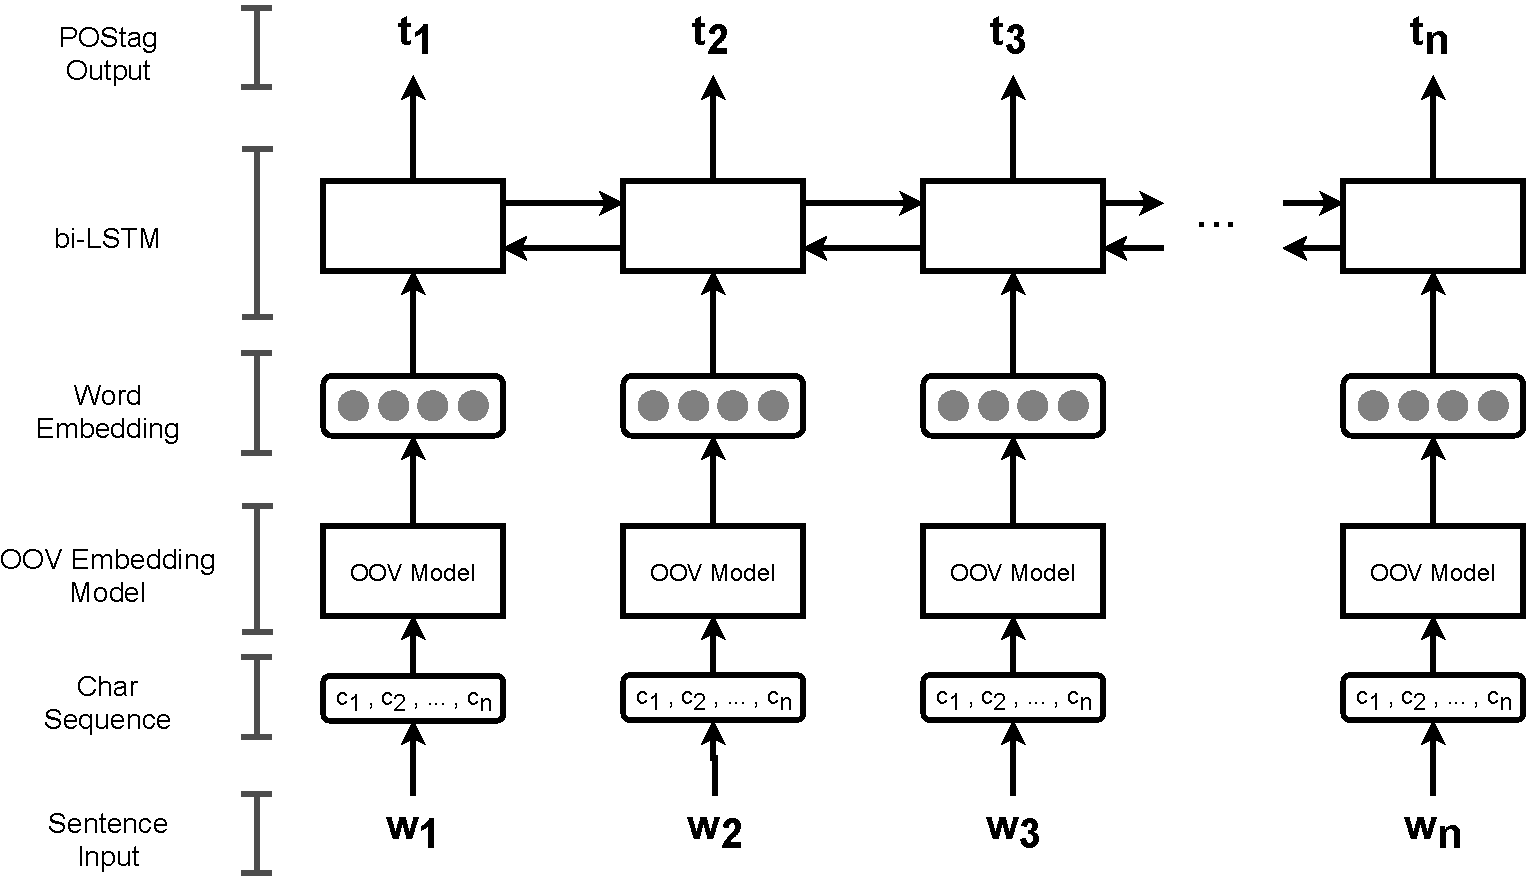
\includegraphics[width=.8\linewidth]{images/postag.pdf}
            \caption{Pos-tagging Process}
            \label{fig:postag}
        \end{figure}
 
    \subsection{Word Similarity Tasks}
        Word similarity tasks is basically task to evaluate the
        similarities between two words based on human given scores. In
        practice, several human subjects were given pairs of words and
        asked to score its similarities. Those scores then will be
        used to determine the agreements between subjects that certain
        word pairs have stronger connection and the others are weaker.
        In order to calculate the agreements between the OOV generated
        embedding and the data that is scored by human, Spearman's
        rank correlation coefficient is used. Firstly, given a pair
        $(w_1, w_2)$, the cosine distance of the embedding
        $\tilde{e}_1$ and $\tilde{e}_2$ based on the generated
        embedding from OOV model for $w_1$ and $w_2$ calculated
        respectively using the following equation,

        \begin{equation}
            \label{eq:cosinesim}
            CosineSimilarity(e_1, e_2) = \frac{e_1 \cdot e_2}{\Vert e_1 \Vert \Vert e_2 \Vert}
        \end{equation}

        After all of the cosine distance for all pairs are calculated,
        Spearman rank's correlation from the dataset and the generated
        embedding are calculated by using equation \ref{eq:spearman}
        and by using equation \ref{eq:spearmantied} when no tied ranks
        exists. The results of both \textsc{Mimick} and the proposed
        model from several word similarity datasets then averaged and
        compared.
        
        \begin{align}
            \label{eq:spearman}
            \rho    &= \ddfrac{n\sum_{i=1}^n u_i v_i - \Bigg( \sum_{i=1}^n u_i \Bigg) \Bigg( \sum_{i=1}^n v_i \Bigg)}{\sqrt{\Bigg[ n \sum_{i=1}^n u_i^2 - \Bigg( \sum_{i=1}^n u_i \Bigg)^2 \Bigg] \Bigg[ n \sum_{i=1}^n v_i^2 - \Bigg( \sum_{i=1}^n v_i \Bigg)^2 \Bigg] }}\\
            \label{eq:spearmantied}            
                    &= 1 - \ddfrac{6 \sum_{i=1}^n d_i^2}{n(n^2 - 1)}\ \text{where}\ d_i = u_i - v_i
        \end{align}
